%%
% Please see https://bitbucket.org/rivanvx/beamer/wiki/Home for obtaining beamer.
%%
\documentclass{beamer}
\usetheme{Warsaw}
\usecolortheme{orchid}
\usepackage[font=scriptsize]{caption}



\title{Spectral rigidity of some arithmetic surfaces}
\author{Justin Katz}
\institute{Purdue University}


\begin{document}
\frame{\titlepage}



\begin{frame}
	\frametitle{Spectra: rigidity and flexibility}
	In general, you cannot hear the shape of a drum: 
	\pause
	\begin{center}
		\begin{figure}
				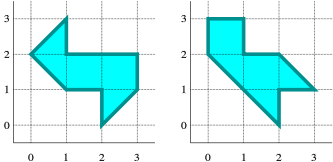
\includegraphics[scale=.4]{isospectralDrums}  
				\caption{Some isospectral drums}
		\end{figure}
	\end{center}
	\pause 
	Soft speculation: sufficiently special drums should sound unique.
	\pause
	\begin{center}
		\begin{figure}		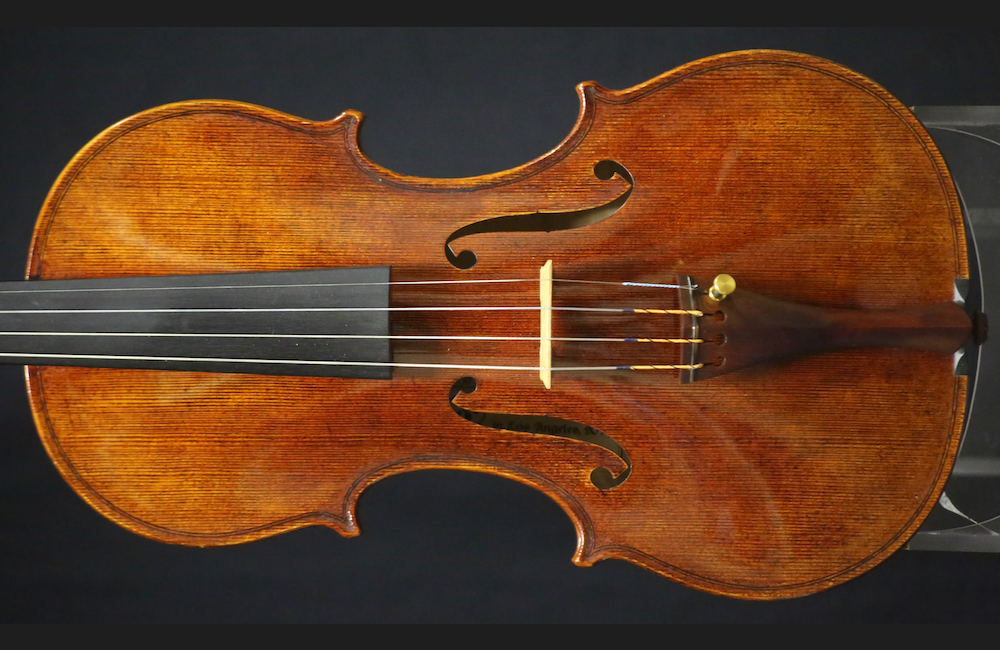
\includegraphics[scale=.18]{fancyViolin.png}
			\caption{A very special (expensive) drum}
		\end{figure}
	\end{center}
\end{frame}

\begin{frame}
	\frametitle{Hurwitz surfaces: the most symmetric of drums}
	A Hurwitz surface is a compact hyperbolic Riemann surface $X$ of genus $g$ such that $|\operatorname{Aut}(X)| = 84(g-1)$. 
	\pause 	
	\begin{center}
		\begin{figure}
		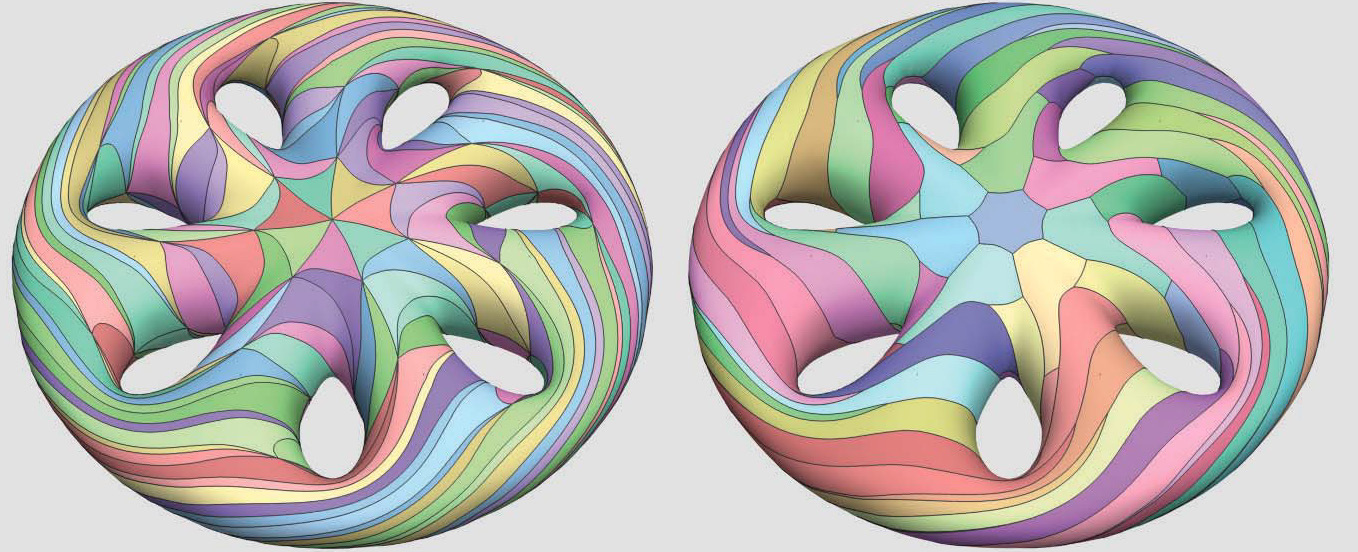
\includegraphics[scale=.18]{vanWijkGenus7.jpg}
			\caption{A genus $7$ Hurwitz (Macbeath) surface 
				\cite{vanwijk2009}}
		\end{figure}
	\end{center}
\end{frame}


\begin{frame}
	\frametitle{Specific speculation}
	\bigskip
	  In \cite{reid2014},  Alan asked whether Hurwitz surfaces are determined up to isometry by their spectrum. 
	\pause
	\begin{figure}
		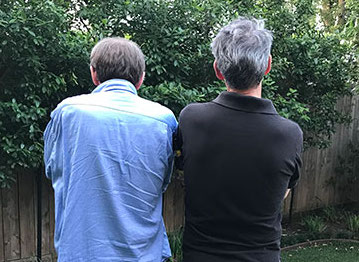
\includegraphics[scale=.4]{Alan_Darren.jpeg}
			\caption{not a genus $7$ Hurwitz (Macbeath) surface}
		\end{figure}
	The following theorem answers in the affirmative infinitely many times (though, not all!)
\end{frame}

\begin{frame}
	The standard setup for arithmetic hyperbolic surfaces:
	\pause
	\begin{itemize} 
		\item $k$ is a totally real number field, with ring of integers $R_k$ \pause
		\item $B$ is an indefinite quaternion algebra over $k$, split over a unique real place. \pause
		\item $\mathcal{O}$ is a maximal order in $B$, and $\mathcal{O}^1$ its group of norm $1$ units.  \pause
		\item $\Gamma(1)$ is the image of $\mathcal{O}^1$ in $\operatorname{PSL}(2,\mathbb{R})$ (an arithmetic lattice) \pause
		\item For an ideal $I$ of $R_k$, let $\Gamma(I)$ be the kernel of the reduction map $\Gamma(1) \to \operatorname{PSL}(2,R_k/I)$.
	\end{itemize}
\end{frame}

\begin{frame} 
	\begin{theorem}[McReynolds, Katz \emph{in progress}]
		Suppose that $B$ has \textbf{type number 1}. Then for all but finitely many primes $\mathcal{P}$ of $R_k$,  and for all $n\geq 0$, the hyperbolic surface $\Gamma(\mathcal{P}^{n}) \backslash \mathbb{H}$ is spectrally rigid.   
	\end{theorem}
	
	\bigbreak
	The standard setup for arithmetic hyperbolic surfaces:
	\begin{itemize} 
		\item $k$ is a totally real number field, with ring of integers $R_k$
		\item $B$ is an indefinite quaternion algebra over $k$, split over a unique real place.
		\item $\mathcal{O}$ is a maximal order in $B$, and $\mathcal{O}^1$ its group of norm $1$ units.
		\item $\Gamma(1)$ is the image of $\mathcal{O}^1$ in $\operatorname{PSL}(2,\mathbb{R})$ (an arithmetic lattice)
		\item For an ideal $I$ of $R_k$, let $\Gamma(I)$ be the kernel of the reduction map $\Gamma(1) \to \operatorname{PSL}(2,R_k/I)$.
	\end{itemize}
\end{frame}

\begin{frame}
	\frametitle{Examples:}
	\begin{itemize}
		\item If the field $k$ has class number $1$ (or more generally, the class group has no $2$-torsion), then the type number hypothesis is satisfied for every indefinite quaternion algebra $B$ over $k$ (provided $B$ is split over a unique real place) \pause
		\item In particular, this theorem applies to all  \emph{rational} indefinite quaternion algebras: \pause \textbf{it applies to $\operatorname{PSL}(2,\mathbb{Z})$ and its principal congruence subgroups!}  \pause
		\item Hurwitz surfaces arise from normal subgroups of the $2,3,7$ triangle group, which arises as the norm $1$ units of a quaternion algebra over the field $\mathbb{Q}(2 \cos 2 \pi / 7)$, which has class number $1$. Hence  the theorem applies: \textbf{principal congruence Hurwitz surfaces are spectrally rigid.}
	\end{itemize}
\end{frame}


\bibliography{/Users/katz9/Documents/Zotero/exports/myLibrary-[auto-export]}
\bibliographystyle{apalike}


\end{document}


